\section{O problema}
\label{sec:problem}

A execução musical praticada em conjunto é altamente colaborativa. Em gêneros com tendências improvisacionais, como \textit{jazz}, \textit{blues} e \textit{rock}, é comum que hajam um ou mais integrantes que usam como base os ritmos e conjunto de acordes praticados por seus colegas para executar \textit{solos} que reagem de acordo com as mudanças da harmonia. É importante, portanto, que haja um \textit{feedback} fluído entre o improvisador e a base musical para que todos possuam conhecimento se o que está sendo tocado está de acordo com suas intenções.

Em gêneros mais metódicos, como música clássica, onde os músicos seguem instruções de partituras e um condutor, reação à mudanças é menos importante. Porém, ainda é necessária a garantia que todos estejam tocando em sincronia uns com os outros. Para o condutor, é importante que possua ciência do que está sendo executado por cada conjunto de instrumentos, de forma a garantir totalmente a harmonia e ritmo entre as partes \cite{conductor_role}.

A tolerância máxima de latência na prática musical é bastante restritiva. Para instrumentos digitais, Wessel e Wright sugerem não mais que 10 ms entre o \textit{input} do artista e o \textit{output} do som \cite{digital_instrument_latency}. Carôt, por sua vez, define o objetivo de alcançar latências menores que 30 ms para que os músicos tenham a sensação de estarem tocando em um mesmo ambiente físico \cite{carot_low_latency}. Ele observa também que, após esse limite, os artistas mudam a forma sobre como performam para adaptarem-se.

Quando performado em conjunto no mesmo ambiente físico, normalmente não há percepção de latência entre os integrantes. Tal latência é baseada na velocidade em que o som se propaga no ar em temperatura ambiente que, em uma velocidade de 343,2 m/s \cite{speed_of_sound}, produz cerca de 3 ms de atraso por metro de distância entre cada músico, sendo, portanto, negligenciável para a sensação de fluidez dos músicos.

No entanto, em ambientes colaborativos \textit{online}, outros fatores podem interferir na latência total. Primeiramente, para que os computadores do participantes consigam processar o áudio, é necessário que haja uma conversão dos sinais analógicos para digitais. Tal processamento consome cerca de 1 ms \cite{how_low_can_you_go}, podendo ser negligenciado. Uma vez convertidos, os sinais precisam ser escritos e lidos no \textit{buffer} em memória, processo que dura entre 10 ms e 12 ms \cite{how_low_can_you_go}, dependendo do poder de processamento das máquinas envolvidas. Ambos processos ocorrem no lado do transmissor (aquele que produz a música) e dos receptores, portanto, dobrando o tempo total.

O maior gargalo, no entanto, pode ocorrer na transmissão dos pacotes de dados via Internet. Devido à abordagem de ``melhor esforço'' na qual a Internet foi originalmente projetada - sob a suposição de que não é possível garantir o recebimento de todos os pacotes transmitidos - protocolos de transmissão de voz como \textit{VoIP} (\textit{Voice over Internet Protocol}) e serviços provedores videoconferências necessitam implementar medidas compensatórias, como grandes \textit{buffers} de rede e retransmissão de pacotes. Tais medidas, consequentemente, garantem a corretude dos dados transmitidos, sob o custo do aumento na latência total \cite{carot_low_latency}.

\begin{figure}[htbp]
\centering
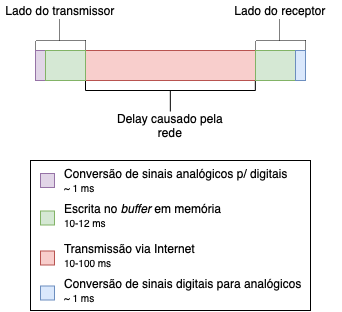
\includegraphics[width=0.5\textwidth]{images/streaming-latency.png}
\caption{Latências de cada fase do processo de \textit{streaming} de áudio pela Internet}
\label{fig:streaming_latencies}
\end{figure}

Aplicações comerciais de videoconferências, como o \textit{Zoom}, \textit{Google Meet} e \textit{FaceTime} também  possuem sensibilidade de tempo para manter conversas compreensíveis - a \textit{Cisco} define a latência máxima aceitável de uma implementação \textit{VoIP} em até 150 ms \cite{cisco}. Este limite pode ser alcançado por conexões de velocidades medianas, mesmo considerando fatores como processamento de áudio, distância entre os participantes e infraestruturas de rede compartilhadas. No entanto, para a prática colaborativa musical, onde tolerância máxima é bastante restrita, o uso de aplicações que implementam \textit{VoIP} mostra-se inviável.

A tolerância de atraso para a performance musical, portanto, é um dos maiores desafios na implementação de ambientes colaborativos musicais \textit{online}. Afinal, mesmo considerando a velocidade da luz no vácuo - aproximadamente 300 km/ms \cite{speed_of_light} - a menor distância possível para obter uma latência ótima de 10 ms é de aproximadamente 3.000 km - um pouco mais que a distância entre Recife, PE e Porto Alegre, RS\footnote{Distância calculada utilizando o Google Maps. ©2021 Google}.

Dessa forma, métodos para redução da latência entre os participantes - ou a sensação de sua existência - possuem suma relevância para músicos. Em contextos onde a presença física dos participantes não é possível de se obter, como o recomendado pelo distanciamento social como método de prevenção de contaminação na Pandemia de COVID-19, a colaboração \textit{online} é o único meio onde músicos conseguem tocar em conjunto.
